\documentclass[11pt]{article}

\usepackage{times,mathptm}
\usepackage{pifont}
\usepackage{exscale}
\usepackage{latexsym}
\usepackage{amsmath}
\usepackage{epsfig}
\usepackage{alltt}
\usepackage{tikz}
\usetikzlibrary{trees,shapes,snakes}

\textwidth 6.5in
\textheight 9in
\oddsidemargin -0.1in
\topmargin -0.6in

\parindent 0pt
\parskip 0pt

\begin{document}
\rightline{Jessica Chen}
\rightline{Collaborators: Andrew Jones}
\begin{LARGE}
\centerline {\bf CSCI 303: Algorithms, HW 10}
\end{LARGE}
\vskip 0.25cm
\centerline{Due: 3:30 pm, Wednesday, 11/14}

\begin{enumerate}
\item Problem 1\\
\begin{enumerate}
\item Remove (a,c), and add b, and c to the heap.\\
\begin{tabular}{c|ccccccc|}
Adjacency& Edge, Cost\\\hline
a& b, 6 & c, 5\\
b&a, 6& c, 9& e, 13\\
c&a, 5&b, 9& d, 16& f, 15\\
d& c, 16& e, 12&\\
e&b, 13&d, 12& g, 8\\
f& c, 15& g, 2\\
g& e, 8&f, 2
\end{tabular}\\
\begin{tabular}{ccccccccccc}
Minimum Binary Heap\\\hline
&0&1&2&3\\
&(a, c), 5 & (a, b), 6\\
\end{tabular}\\
\begin{tabular}{c|ccccccc|}
$v$& Known& $d_v$ & $p_v$\\\hline
a& T & 0& 0\\
b&F & 6 & a\\
c&F & 5 & a\\
d&F & $\infty$ & 0\\
e&F & $\infty$ & 0\\
f&F & $\infty$ & 0\\
g&F & $\infty$ & 0
\end{tabular}\\
\begin{tabular}{c|ccccccc|}
Adjacency& Edge, Cost\\\hline
a& c, 5\\
\end{tabular}\\
% Set the overall layout of the tree
\tikzstyle{level 1}=[level distance=3.5cm, sibling distance=3.5cm]
\tikzstyle{level 2}=[level distance=3.5cm, sibling distance=2cm]
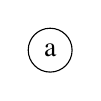
\begin{tikzpicture}[grow=right, sloped]
\node [circle, draw]{a};
\end{tikzpicture}

\item Remove c from the heap, and add it's adjacent nodes to the heap.\\
\begin{tabular}{ccccccccccc}
Minimum Binary Heap\\\hline
&0&1&2&3\\
& (a, b), 6& (c, f), 15& (c, d), 16\\
\end{tabular}\\
\begin{tabular}{c|ccccccc|}
$v$& Known& $d_v$ & $p_v$\\\hline
a& T & 0& 0\\
b&F & 6 & a\\
c&T & 5 & a\\
d&F & 16 & c\\
e&F & $\infty$ & 0\\
f&F & 15 & f\\
g&F & $\infty$ & 0
\end{tabular}\\
\begin{tabular}{c|ccccccc|}
Adjacency& Edge, Cost\\\hline
a& c, 5\\
c&a, 5&\\
\end{tabular}\\
% Set the overall layout of the tree
\tikzstyle{level 1}=[level distance=1cm, sibling distance=3.5cm]
\tikzstyle{level 2}=[level distance=3.5cm, sibling distance=2cm]
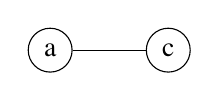
\begin{tikzpicture}[grow=right, sloped]
\node [circle, draw]{a}
	child {node [circle,draw] {c}};
\end{tikzpicture}

\item Remove (a, b) from the heap, and add it's adjacent nodes to the heap.\\
\begin{tabular}{ccccccccccc}
Minimum Binary Heap\\\hline
&0&1&2&3\\
& (b, e), 13& (c, f), 15& (c, d), 16\\
\end{tabular}\\
\begin{tabular}{c|ccccccc|}
$v$& Known& $d_v$ & $p_v$\\\hline
a& T & 0& 0\\
b&T & 6 & a\\
c&T & 5 & a\\
d&F & 16 & c\\
e&F & 13 & b\\
f&F & 15 & f\\
g&F & $\infty$ & 0
\end{tabular}\\
\begin{tabular}{c|ccccccc|}
Adjacency& Edge, Cost\\\hline
a& b, 6 & c, 5\\
b&a, 6&\\
c&a, 5&\\
\end{tabular}\\
% Set the overall layout of the tree
\\
\tikzstyle{level 1}=[level distance=1cm, sibling distance=3cm]
\tikzstyle{level 2}=[level distance=3.5cm, sibling distance=2cm]
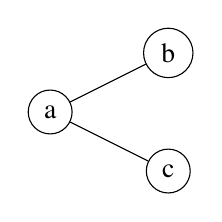
\begin{tikzpicture}[grow=right, sloped]
\node [circle, draw]{a}
	child {node [circle,draw] {c}}
	child {node [circle,draw] {b}};
\end{tikzpicture}


\item Remove (b, e), and add it's adjacent nodes to the heap.\\
\begin{tabular}{ccccccccccc}
Minimum Binary Heap\\\hline
&0&1&2&3\\
&(e, g), 8&(e, d), 12& (c, f), 15& \\
\end{tabular}\\
\begin{tabular}{c|ccccccc|}
$v$& Known& $d_v$ & $p_v$\\\hline
a&T & 0 & 0\\
b&T & 6 & a\\
c&T & 5 & a\\
d&F & 12 & e\\
e&T & 13 & b\\
f&F & 15 & c\\
g&F & 8 & e
\end{tabular}\\
\begin{tabular}{c|ccccccc|}
Adjacency& Edge, Cost\\\hline
a& b, 6 & c, 5\\
b&a, 6&e, 13\\
c&a, 5&\\
e&b, 13\\
\end{tabular}\\
% Set the overall layout of the tree
\\
\tikzstyle{level 1}=[level distance=1cm, sibling distance=3cm]
\tikzstyle{level 2}=[level distance=3.5cm, sibling distance=2cm]
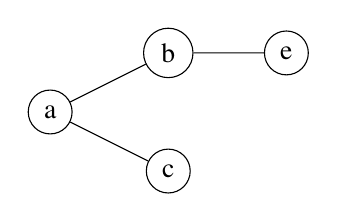
\begin{tikzpicture}[grow=right, sloped]
\node [circle, draw]{a}
	child {node [circle,draw] {c}}
	child {node [circle,draw] {b}
			child {node [circle,draw] {e}}};
\end{tikzpicture}

\item Remove (e, g), and add it's adjacent nodes to the heap.\\
\begin{tabular}{ccccccccccc}
Minimum Binary Heap\\\hline
&0&1&2&3\\
&(g, f), 2&(e, d), 12& \\
\end{tabular}\\
\begin{tabular}{c|ccccccc|}
$v$& Known& $d_v$ & $p_v$\\\hline
a&T & 0 & 0\\
b&T & 6 & a\\
c&T & 5 & a\\
d&F & 12 & e\\
e&T & 13 & b\\
f&F & 2 & g\\
g&T & 8 & e
\end{tabular}\\
\begin{tabular}{c|ccccccc|}
Adjacency& Edge, Cost\\\hline
a& b, 6 & c, 5\\
b&a, 6&e, 13\\
c&a, 5&\\
e&b, 13& g, 8\\
g& e, 8\\
\end{tabular}\\
% Set the overall layout of the tree
\\
\tikzstyle{level 1}=[level distance=1cm, sibling distance=3cm]
\tikzstyle{level 2}=[level distance=3.5cm, sibling distance=2cm]
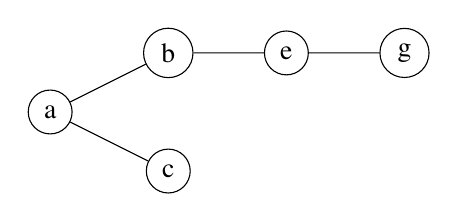
\begin{tikzpicture}[grow=right, sloped]
\node [circle, draw]{a}
	child {node [circle,draw] {c}}
	child {node [circle,draw] {b}
			child {node [circle,draw] {e}
				child {node [circle,draw] {g}}}};
\end{tikzpicture}

\item Remove (g, f), and add it's adjacent nodes to the heap.\\
\begin{tabular}{ccccccccccc}
Minimum Binary Heap\\\hline
&0&1&2&3\\
&(e, d), 12 \\
\end{tabular}\\
\begin{tabular}{c|ccccccc|}
$v$& Known& $d_v$ & $p_v$\\\hline
a&T & 0 & 0\\
b&T & 6 & a\\
c&T & 5 & a\\
d&F & 12 & e\\
e&T & 13 & b\\
f&T & 2 & g\\
g&T & 8 & e
\end{tabular}\\
\begin{tabular}{c|ccccccc|}
Adjacency& Edge, Cost\\\hline
a& b, 6 & c, 5\\
b&a, 6&e, 13\\
c&a, 5&\\
e&b, 13& g, 8\\
f& g, 2\\
g& e, 8& f, 2\\
\end{tabular}\\
% Set the overall layout of the tree
\\
\tikzstyle{level 1}=[level distance=1cm, sibling distance=3cm]
\tikzstyle{level 2}=[level distance=3.5cm, sibling distance=2cm]
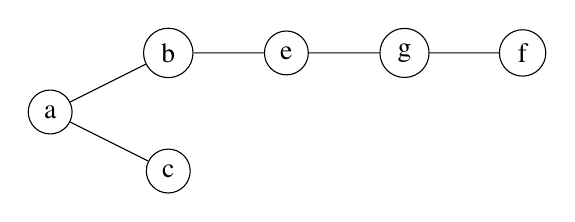
\begin{tikzpicture}[grow=right, sloped]
\node [circle, draw]{a}
	child {node [circle,draw] {c}}
	child {node [circle,draw] {b}
			child {node [circle,draw] {e}
				child {node [circle,draw] {g}
					child {node [circle,draw] {f}}}}};
\end{tikzpicture}

\item Remove (e, d), and add it's adjacent nodes to the heap.\\
\begin{tabular}{ccccccccccc}
Minimum Binary Heap\\\hline
&0&1&2&3&\\
&(e, d), 12 \\
\end{tabular}\\
\begin{tabular}{c|ccccccc|}
$v$& Known& $d_v$ & $p_v$\\\hline
a&T & 0 & 0\\
b&T & 6 & a\\
c&T & 5 & a\\
d&T & 12 & e\\
e&T & 13 & b\\
f&T & 2 & g\\
g&T & 8 & e
\end{tabular}\\
\begin{tabular}{c|ccccccc|}
Adjacency& Edge, Cost\\\hline
a& b, 6 & c, 5\\
b&a, 6&e, 13\\
c&a, 5&\\
d& e, 12\\
e&b, 13& g, 8& d, 12\\
f& g, 2\\
g& e, 8& f, 2\\
\end{tabular}\\
% Set the overall layout of the tree
\\
\tikzstyle{level 1}=[level distance=1cm, sibling distance=3cm]
\tikzstyle{level 2}=[level distance=3.5cm, sibling distance=2cm]
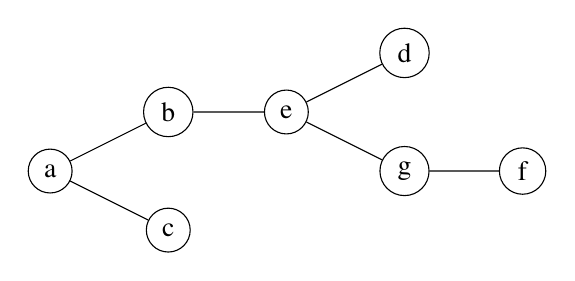
\begin{tikzpicture}[grow=right, sloped]
\node [circle, draw]{a}
	child {node [circle,draw] {c}}
	child {node [circle,draw] {b}
			child {node [circle,draw] {e}
				child {node [circle,draw] {g}
					child {node [circle,draw] {f}}}
				child {node [circle,draw] {d}}}};
\end{tikzpicture}


\end{enumerate}
\item Problem 2\\
Use Prim's algorithm, but instead of picking the minimum pick the edge with the max cost each time(use a maximum binary heap). It's not harder because you are just changing whether you choose the min or the max.
\item Problem 3\\
\begin{tabular}{l||c|c|c}
Selection algorithm&$k=1$ & $k=\lceil \frac{n}{2} \rceil$& $k=n$\\\hline \hline
sort select& O($n^2$) or O($nlogn$)& O($n^2$) or O($nlogn$) &O($n^2$) or O($nlogn$)\\\hline
partial sort select& O($n$) & O($n^2$) & O($nlogn$)\\\hline
minimum binary heap select&  O($n$)& O($nlogn$)  & O($nlogn$)\\\hline
partial maximum binary heap select & O($n$) &O($nlogn$) &O($n$) 
\end{tabular}
\end{enumerate}
\end{document}